\documentclass{beamer}

\usepackage{anyfontsize}
\usepackage{listings}
\usepackage{color}
\usepackage{inconsolata}
\usepackage{tikz}
\usepackage{hyperref}
%\usepackage{textpos}
% OL%
\usetheme{loosekit}
\beamertemplatenavigationsymbolsempty

\definecolor{mygreen}{rgb}{0,0.6,0}
\definecolor{mygray}{rgb}{0.5,0.5,0.5}
\definecolor{mymauve}{rgb}{0.58,0,0.82}

\usetikzlibrary{shapes.misc}

\newcommand{\KeY}{Ke\kern-.1em Y}
\newcommand{\kit}[1]{\textcolor{kit-green100}{#1}}
\newcommand{\kitblue}[1]{\textcolor{kit-blue100}{#1}}


\lstset{ 
  backgroundcolor=\color{white},   % choose the background color; you must add \usepackage{color} or \usepackage{xcolor}; should come as last argument
  basicstyle=\tiny\ttfamily,               % the size of the fonts that are used for the code
  breakatwhitespace=false,         % sets if automatic breaks should only happen at whitespace
  breaklines=true,                 % sets automatic line breaking
  captionpos=b,                    % sets the caption-position to bottom
  commentstyle=\color{green},    % comment style
  deletekeywords={...},            % if you want to delete keywords from the given language
  %escapeinside={@*}{*@)},          % if you want to add LaTeX within your code
  extendedchars=true,              % lets you use non-ASCII characters; for 8-bits encodings only, does not work with UTF-8
  %firstnumber=1000,                % start line enumeration with line 1000
  frame=single,	                   % adds a frame around the code
  keepspaces=true,                 % keeps spaces in text, useful for keeping indentation of code (possibly needs columns=flexible)
  keywordstyle=\color{blue},       % keyword style
  language=Java,                 % the language of the code
  alsoletter={\\},
  morekeywords={*,invariant,\\forall,requires,ensures,normal_behaviour,ghost,model,\\old,\\result,assignable,\\in,accessible},            % if you want to add more keywords to the set
  %numbers=left,                    % where to put the line-numbers; possible values are (none, left, right)
  numbersep=5pt,                   % how far the line-numbers are from the code
  %numberstyle=\tiny\color{mygray}, % the style that is used for the line-numbers
  rulecolor=\color{blue},         % if not set, the frame-color may be changed on line-breaks within not-black text (e.g. comments (green here))
  showspaces=false,                % show spaces everywhere adding particular underscores; it overrides 'showstringspaces'
  showstringspaces=false,          % underline spaces within strings only
  showtabs=false,                  % show tabs within strings adding particular underscores
  %stepnumber=2,                    % the step between two line-numbers. If it's 1, each line will be numbered
  %stringstyle=\color{mymauve},     % string literal style
  %tabsize=2,	                   % sets default tabsize to 2 spaces
  %title=\lstname                   % show the filename of files included with \lstinputlisting; also try caption instead of title
  deletecomment={[l]//},%
  deletecomment={[s]{/*}{*/}},%
}


\title{The \KeY-verified Verified Keyserver}

\subtitle{VerifyThis Long Term Challenge}

\date{27 April 2020}
\author[de Gouw, Ulbrich, Weigl]%
  {Stijn de Gouw (Open University, NL),
   Mattias Ulbrich, Alexander Weigl}

\institute{Institute of Theoretical Informatics}

\begin{document}

% OL%\selectlanguage{english}

\begin{frame}
\titlepage
\end{frame}

\begin{frame}{Our program verifier \KeY}
  \vspace{-1.5cm}
  \begin{center}
    \begin{tikzpicture}
      \node at (0,0) { 
\includegraphics[height=8cm]{key} };
      \node at (-2.5,2.5) {\large Deductive verification};
      \node[text width=3cm] at (-4.5,.5) {\large Java Modeling\\Language (JML)};
      \node[text width=3cm] at (4,-1.5) {\large Modular\\Reasoning};
      \node at (-3.5,-1.5) {\large Mostly automatic};
      \node at (2,2.5) {\large 100\% Java Card};
      \node at (-2,-2.5) {\large User Interaction Concepts};
      %\node at (2,-3) {\large Secure Information Flow};
      \node at (0,-4) {\footnotesize collaboration with
        TU Darmstadt and Chalmers University, Gothenburg};
    \end{tikzpicture}
  \end{center}\vspace{-1ex}
\end{frame}

\begin{frame}
  \frametitle{Modelling HAGRID in \KeY}

  We present two formalisations of the HAGRID framework as spec'ed and
  verif'ed Java implementations:
  \pause
  
  \begin{block}{The \textbf{array} model}
%  \footnotesize
    \begin{itemize}
    \item uses arrays to implement database and open requests
    \item specification on these arrays
    \item 70 loc, 90 los, 10 POs, \textbf{fully automatic}
    \end{itemize}
  \end{block}

  \only<1-2>{\it\footnotesize loc/los = lines of code/spec, POs = \# of
    proof obligations}
    
  
  \pause
  \begin{exampleblock}{The \textbf{map} model}
%  \footnotesize
  \begin{itemize}
    \item uses map data structures to implement db and open requests
    \item specification on ADT maps
    \item ``object singularities''
    \item 146 loc, 262 los, 40 POs, \textbf{89 interactions}
    \end{itemize}
  \end{exampleblock}
  % \tikz[overlay, text width=10cm] \node at (11.7,2) {\it\footnotesize loc/los = lines of code/spec\\POs = \# of proof obligations};
  
\end{frame}

\section{Array Model: Class Overview}
\begin{frame}
    \frametitle{Array Model: Overview}
    \begin{columns}
      \begin{column}{.7\textwidth}
        \begin{itemize}
          \item Backend of a Verifying Keyserver
          \begin{itemize}
            \item retrieving of public keys
            \item \emph{verified} adding of entries
            \item \emph{verified} deletion of entries
          \end{itemize}
          \item Simplifications
          \begin{itemize}
            \item All data types are (array of) \texttt{int}'s.
            \item In memory map-like storage
            \item Maps are represented \\by a key and value array.
          \end{itemize}
          \item \href{https://github.com/KeYProject/verifythis-ltc-2020/blob/master/simplified/Keyserver.java}%
          {simplified/Keyserver.java}
        \end{itemize}
      \end{column}
      \begin{column}{.45\textwidth}
        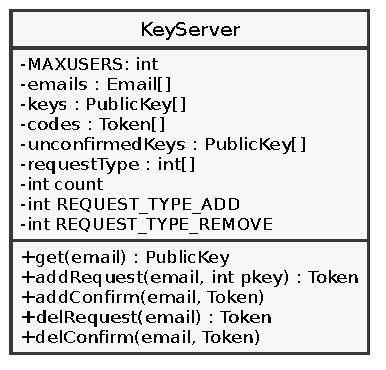
\includegraphics[width=\textwidth]{simplified_uml.pdf}
      \end{column}
    \end{columns}
\end{frame}

\begin{frame}[fragile]
    \frametitle{Array Model: Invariants}
    
  \begin{block}{\small ruling out aliasing}
    \vspace{-.5em}
    \begin{lstlisting}
invariant emails != keys && emails != codes && emails != unconfirmedKeys;
invariant emails != requestType && keys != codes && keys != unconfirmedKeys;
invariant keys != requestType && codes != unconfirmedKeys && codes != requestType;
invariant unconfirmedKeys != requestType;\end{lstlisting}
  \end{block}
  \vspace{-1em}
  \begin{block}{\small All arrays are non-null and have the same length (\# of users)}
  \vspace{-.5em}
  \begin{lstlisting}
invariant emails != null && keys != null && codes != null;
invariant unconfirmedKeys != null && requestType != null;
invariant emails.length == MAXUSERS && keys.length == MAXUSERS;
invariant codes.length == MAXUSERS && unconfirmedKeys.length == MAXUSERS;
invariant requestType.length == MAXUSERS;\end{lstlisting}
  \end{block}
  \vspace{-1em}
  \begin{block}{\small Number of users is bounded}
  \vspace{-.5em}
\begin{lstlisting}
invariant 0 <= count && count <= MAXUSERS;\end{lstlisting}
  \end{block}
  \vspace{-1em}
\begin{block}{\small Emails are unique}
  \vspace{-.5em}
\begin{lstlisting}  
invariant (\forall int i,j ; 
                0 <= i && i < j && j < count; 
                    emails[i] != emails[j]);\end{lstlisting}
  \end{block}
\end{frame}



\lstset {
  basicstyle=\fontsize{7.2}{8.64}\ttfamily,
}


\begin{frame}[fragile]
    \frametitle{Array Model: Informal Method Contract}
    \begin{block}{Informal Contract: \texttt{addRequest(Email, PublicKey)}}
      Stores request to add the given key for the specified user. The key still
      needs to be confirmed with \texttt{\#addConfirm(Email, Token)}. Does nothing if
      the specified user does not exist.
     
    \begin{itemize}
      \item \texttt{id} -- email of the user
      \item \texttt{pkey} -- public key to added after confirmation
      \item \textbf{returns} the array index where the data is stored
    \end{itemize}
     
    \end{block}

    \newcommand{\nlc}[1]{\textcolor{green!60!black}{// #1}}

    \begin{lstlisting}[escapechar=@]
public int addRequest(int id, int pkey) {
  int pos = posOfId(id);               @ \nlc{find the entry in the current} @
  if(pos < 0) { pos = count++; }       @ \nlc{not found, use an empty entry}  @
  emails[pos] = id;                    @ \nlc{store user's email}@
  codes[pos] = random();               @ \nlc{generate/store the auth. token}@
  unconfirmedKeys[pos] = pkey;         @ \nlc{store the key in a additional list}@
  requestType[pos] = REQUEST_TYPE_ADD; @ \nlc{entry is an addition} @
  return pos;                          @ \nlc{! return the \textbf{position} of the entry} @
}\end{lstlisting}

\end{frame}

\begin{frame}[fragile]
    \frametitle{Array model: Formal Method Contract}
    \vspace{-1em}
    \begin{exampleblock}{}
    \vspace{-.5em}
\begin{lstlisting}
/*@ public normal_behaviour

  @ requires count < MAX USERS;
  
  @ ensures 0 <= \result;

  @ ensures count == \old(count) && \result < count
        ||  count == \old(count) + 1 && \result == count - 1;

  @ ensures emails[\result] == id && unconfirmedKeys[\result] == pkey
    &&  codes[\result] > 0 && requestType[\result] == REQUEST_TYPE_ADD;

  @ ensures (\forall int i; 0<=i && i<count;
             (emails[i] == (i == \result ? id : \old(emails[i])))
     && (unconfirmedKeys[i] ==
                 (i == \result ? pkey : \old(unconfirmedKeys[i])))
     && (i != \result ==> (codes[i] == \old(codes[i])))
     && (i != \result ==> (requestType[i] == \old(requestType[i]))));

  @ assignable emails[*], unconfirmedKeys[*],
               codes[*],  requestType[*],     count;
*/
\end{lstlisting}
\end{exampleblock}
\end{frame}


%%
%% -- the map model --
%%

\lstset {
  basicstyle=\footnotesize\ttfamily,
}

\begin{frame}
  \frametitle{The map model}
  \centering  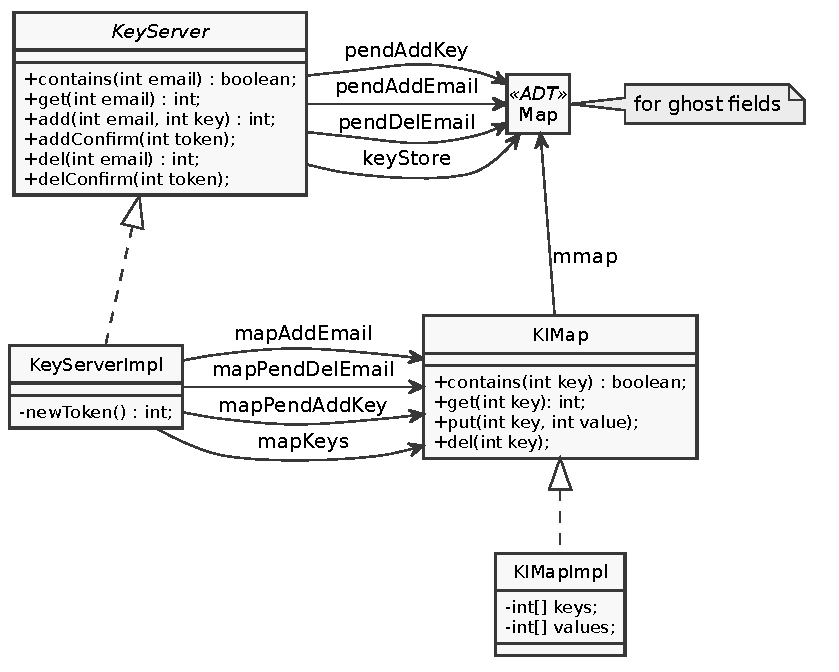
\includegraphics[height=.9\textheight]{imap}
\end{frame}

\begin{frame}[fragile]
  \frametitle{Confirming a new key}

Original syntax: 
\begin{lstlisting}
/*@ public normal_behavior
  @  requires \dl_inDomain(pendAddEmail, token);
  @  ensures keyStore == 
  @   \dl_mapUpdate(\old(keyStore), 
  @      \dl_mapGet(\old(pendAddEmail), token), 
  @      \dl_mapGet(\old(pendAddKey), token));
  @  ensures pendAddEmail == 
  @   \dl_mapRemove(\old(pendAddEmail), token);
  @  ensures pendAddKey == 
  @   \dl_mapRemove(\old(pendAddKey), token);
  @  ensures pendDelEmail == \old(pendDelEmail);
  @  assignable footprint;
  @*/
public void addConfirm(int token);
\end{lstlisting}
\end{frame}


\begin{frame}[fragile]
  \frametitle{Confirming a new key}
  More mathematical syntax:
\begin{lstlisting}
/*@ public normal_behavior
  @  requires token \in pendAddEmail;
  @
  @  ensures keyStore == \old(keyStore)[
  @    \old(pendAddEmail)[token] <-
  @    \old(pendAddKey)[token]];
  @
  @  ensures pendAddEmail == \old(pendAddEmail) - token;
  @
  @  ensures pendAddKey == \old(pendAddKey) - token;
  @
  @  ensures pendDelEmail == \old(pendDelEmail);
  @ 
  @  assignable footprint;
  @*/
public void addConfirm(int token);
\end{lstlisting}
\end{frame}

\begin{frame}[fragile]{Connecting ghosts and implementation}
\vspace{4.5cm}

\begin{lstlisting}
interface KeyServer {
    ghost \map keyStore; /*...*/ }

class KeyServerImpl implements KeyServer {
    KIMap mapKeys = KIMap.newMap();
    invariant mapKeys.<inv>;
    invariant keyStore == mapKeys.mmap; /*...*/}
\end{lstlisting}
\tikz[overlay] \node at (7.5,5.5) {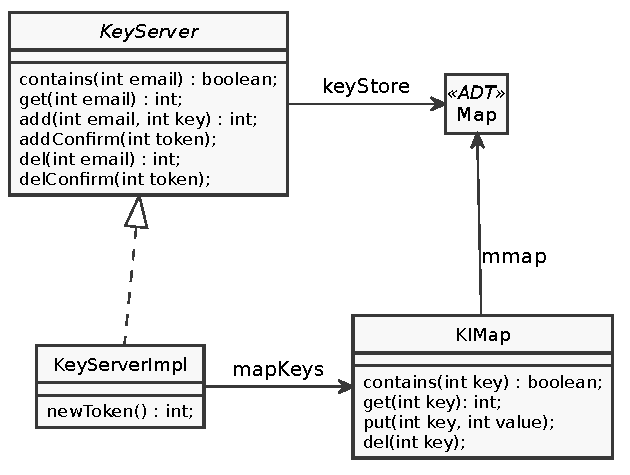
\includegraphics[width=7.5cm]{imap_partial}};
\vspace{10cm}

\end{frame}

\begin{frame}
  \frametitle{Dynamic Frames -- ``Singularities''}
  \begin{alertblock}{}
    \centering Proofs cannot be conducted due to framing problems.
  \end{alertblock}
  \vspace{20cm}
  %overlays!
  % Layer "Heap<1->"
  \pgfdeclareimage[width=\paperwidth]{layer1}{.//heap/layer1}
  \begin{textblock}{1}(0,0)
    \pgfuseimage<1->{layer1}
  \end{textblock}

  % Layer "Objects<2->"
  \pgfdeclareimage[width=\paperwidth]{layer2}{.//heap/layer2}
  \begin{textblock}{1}(0,0)
    \pgfuseimage<2->{layer2}
  \end{textblock}

  % Layer "Intersect<3->"
  \pgfdeclareimage[width=\paperwidth]{layer3}{.//heap/layer3}
  \begin{textblock}{1}(0,0)
    \pgfuseimage<3->{layer3}
  \end{textblock}

  % Layer "Substruct<4->"
  \pgfdeclareimage[width=\paperwidth]{layer4}{.//heap/layer4}
  \begin{textblock}{1}(0,0)
    \pgfuseimage<4->{layer4}
  \end{textblock}

  % Layer "Black Hole<5>"
  \pgfdeclareimage[width=\paperwidth]{layer5}{.//heap/layer5}
  \begin{textblock}{1}(0,0)
    \pgfuseimage<5>{layer5}
  \end{textblock}

  % Layer "Black Lenses<6>"
  \pgfdeclareimage[width=\paperwidth]{layer6}{.//heap/layer6}
  \begin{textblock}{1}(0,0)
    \pgfuseimage<6>{layer6}
  \end{textblock}

  % Layer "Singularities<7->"
  \pgfdeclareimage[width=\paperwidth]{layer7}{.//heap/layer7}
  \begin{textblock}{1}(0,0)
    \pgfuseimage<7->{layer7}
  \end{textblock}

\end{frame}



\begin{frame}[fragile]
  \frametitle{Singularities}
  ~
  \vfill
  
  \begin{minipage}{.7\linewidth}
    \begin{block}{Original class}
\begin{lstlisting}
interface Map {
 //@ ghost \locset footprint;

 //@ model \map mmap;

 /*@ ensures \result == mmap[k];
   @ accessible footprint; */
 int get(int k) {...}

 /*@ ensures mmap == \old(mmap)[k<-v];
   @ assignable footprint; */
  int get(int k, int v) {...}
}
\end{lstlisting}
    \end{block}
  \end{minipage}
  
  \tikz[overlay] \node at (8.8,5) {
    \begin{minipage}{.49\linewidth}
      \begin{exampleblock}<2->{Singularity replacement}
\begin{lstlisting}
interface Map {
 //@ ghost \free footprint;

  ... copy the rest
\end{lstlisting}
        \texttt{\char`\\ free} is uninterpreted sort \\
        ``footprint'' captures the ``state''
      \end{exampleblock}
    \end{minipage}};
\end{frame}

\begin{frame}
  \frametitle{Summary}
  \begin{itemize} \itemsep3ex
  \item \emph{we presented two models:} \\
    one automatic, one pretty interactive
  \item Limitations and open challenges:
    \begin{itemize}
    \item integers instead of strings ($\to$ thesis @ KIT)
    \item linear maps, not hash maps ($\to$ thesis @ OU)
    \item framing, singularities ($\to$ thesis @ KIT)
    \end{itemize}
  \item Long-term goals:
    \begin{itemize}
    \item Specify and verify secure information flow (using \KeY)
    \item Verified data structure library for Java
    \end{itemize}
    \item Spin-off: \emph{ci-tool} for support of KeY in Continuous Integration
     pipelines. \small
    \texttt{https://key-project.org/ci-tool/}
  \end{itemize}
\end{frame}


\end{document}
